\documentclass[amsmath,amssymb, aps, prx, longbibliography, twocolumn]{revtex4-1}

\usepackage{natbib}
\usepackage{graphicx}% Include figure files
\usepackage{dcolumn}% Align table columns on decimal point
\usepackage{bm}
\usepackage[usenames]{color}

\begin{document}

\title{ Detecting non-Fermi liquid transport in the quantum critical region \\ via quantum loop topography}

\author{George Trey Driskell$^1$}
\author{Samuel Lederer$^1$}
\author{Carsten Bauer$^2$}
\author{Simon Trebst$^2$}
\author{Eun-Ah Kim$^1$}
\email{eun-ah.kim@cornell.edu}

\affiliation{%
$^{1}$Department of Physics, Cornell University, Ithaca, New York 14853, USA}%
\affiliation{$^{2}$Institute for Theoretical Physics, University of Cologne, 50937 Cologne, Germany}

\date{\today}

\begin{abstract}

\end{abstract}

\maketitle

%%%%%%%%%%%%%%%%%%%%%%%%%%%%%%%%%%%%%%%%%%%%%%%%%%%%%%%%%%%%%%%%%%
% Introduction
%%%%%%%%%%%%%%%%%%%%%%%%%%%%%%%%%%%%%%%%%%%%%%%%%%%%%%%%%%%%%%%%%%
[1 problem statement: NFL in QC ]
Most often defined by transport in experiment, ubiquitous
\\
\\
\\
\\
\\
\\
\\
\\
\\
\\
\\


[2 literature in sign-free MC]
Transport is hard. "proxies" are not satisfactory.
\\
\\
\\
\\
\\
\\
\\
\\
\\
\\
\\
\\
\\
\\
\\

[3 literature in phase recognition]
Ideal application of ML is where conventional approaches are lacking: such as topological order and NFL.
 \\
 \\
 \\
 \\
 \\
 \\
 \\
 \\
 \\
 \\
 \\
 \\
 \begin{figure} [t]
    \centering
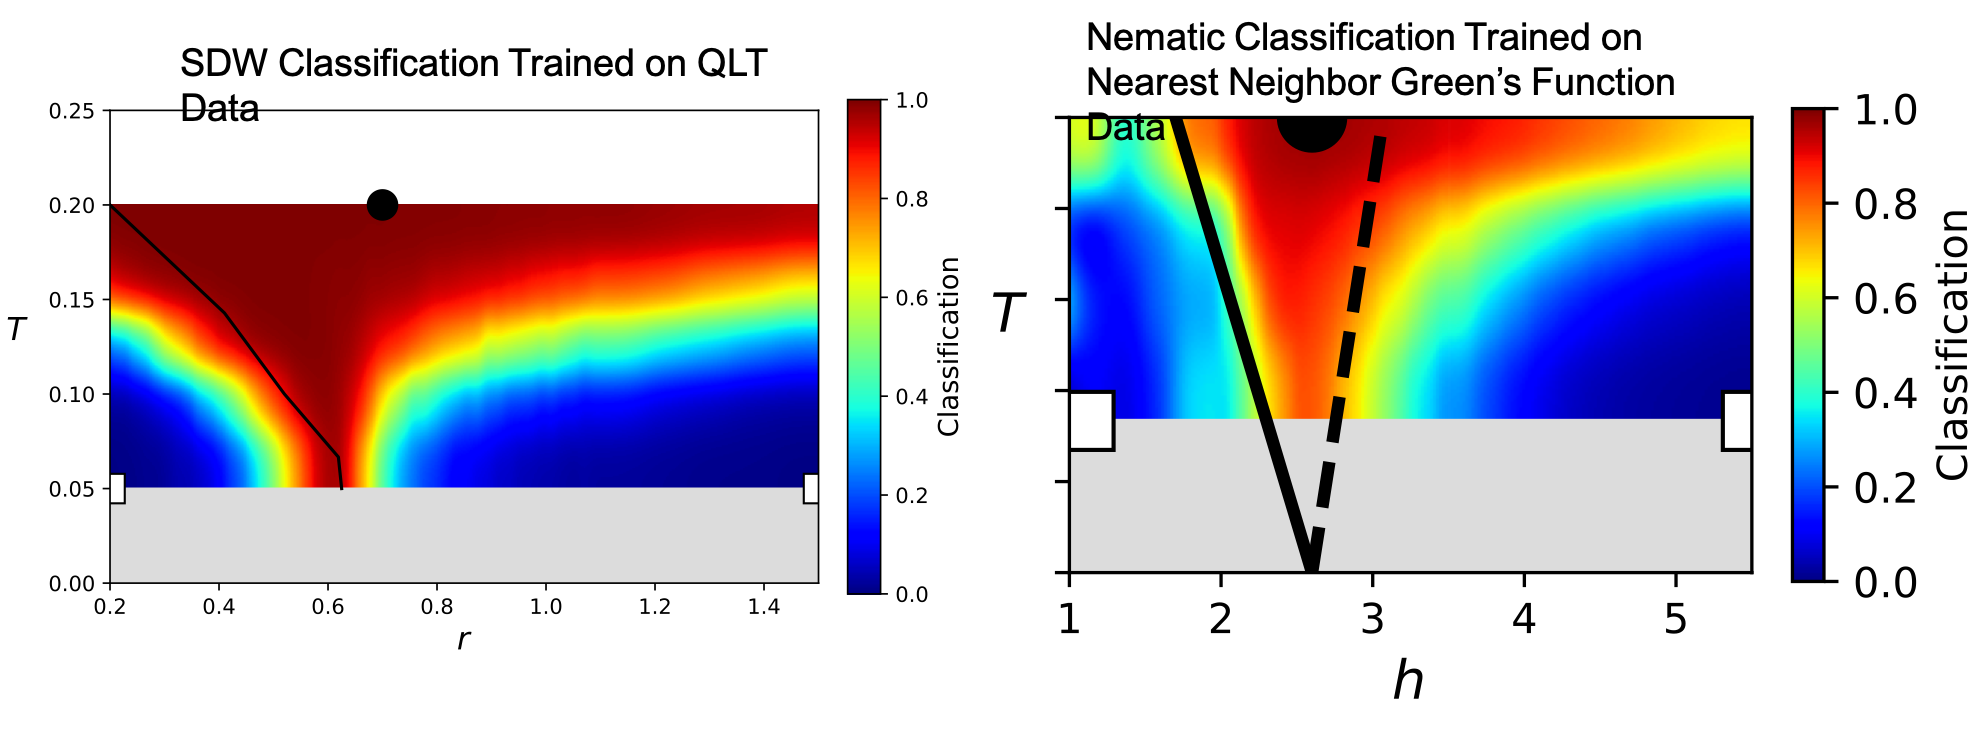
\includegraphics[width=.5\textwidth]{3PT-PDs.png}
    \caption{Caption}
    \label{fig:my_label}
\end{figure}
[4 In this paper - Fig 1] 
\\
\\
\\
\\
\\
\\
\\
\\


[5 Two QCP's to study:]
Their similarities and differences in words.
\\
\\
\\
\\
\\
\\
\\
\\
\\

[6 ML architecture and preprocessing]
\\
\\
\\
\\
\\
\\
\\
\\
\\
\\
\\

[7 SDW model action and what is known]
\\
\\
\\
\\
\\
\\
\\
\\
\\

[8 2pt classification with ]

[9]

[10]

[11]

[12]

[13]

[14]

[15]

[16]

{\it Acknowledgements.--} 
We acknowledge useful discussions with XXX. SL and E-AK acknowledge the support from the U.S. Department of Energy, Office of Basic Energy Sciences, Division of Materials Science and Engineering under Award DE-SC0018946.
The Cologne group acknowledges partial support from the Deutsche Forschungsgemeinschaft (DFG, German Research Foundation) -- Projektnummer 277101999 -- TRR 183 (project B01).
The numerical simulations were performed on the JUWELS cluster at FZ J\"ulich and the CHEOPS cluster at RRZK Cologne.


%\bibliographystyle{apsrev4-1}
%\bibliography{refs,t+X-NSF}
\appendix



\end{document}
